\documentclass[12pt,a4paper, pointlessnumbers, abstraction, headsepline]{scrreprt}

%\usepackage{uarial}
\usepackage{fontspec}
\setmainfont{Arial}
\setsansfont{Arial}
\usepackage[onehalfspacing]{setspace}
\renewcommand\familydefault{\sfdefault}

\usepackage[T1]{fontenc}
\usepackage[utf8]{inputenc}
\usepackage[ngerman]{babel}
\usepackage{graphicx}
\usepackage[left=2cm, right=2cm, bottom=2cm, top=2cm, footskip=1cm]{geometry}
\usepackage{cite}
\usepackage{pdfpages}
\usepackage{pdflscape}
\usepackage[autostyle=true,german=quotes]{csquotes}
%\usepackage{hyperref}
\usepackage{tocloft}

\DeclareMathSizes{12}{12}{12}{12}

\newcommand{\achtung}[1]{\colorbox{red}{#1}}

% --------------------------------------------------------------- 
\makeatletter
\title{Projektarbeit}
\author{\achtung{Vorname Nachname}}
\date{\today}

\addtokomafont{pagenumber}{\sffamily}
\renewcommand{\cftsecfont}{\sffamily}
\renewcommand{\cftsecpagefont}{\sffamily}
\renewcommand{\cftsubsecfont}{\sffamily}
\renewcommand{\cftsubsecpagefont}{\sffamily}

\setkomafont{caption}{\sffamily}
\setkomafont{captionlabel}{\usekomafont{caption}}
\renewcommand{\cftfigfont}{\sffamily}
\renewcommand{\cftfigpagefont}{\sffamily}

\begin{document}
	\titlepage
\begin{center}
% Logo Deckblatt
%\includegraphics[width=9cm]{TH-Logo}\vspace{0.5cm}

\par\end{center}

\noindent \begin{center}
\textsf{\textbf{\Large Dokumentation zu einem praxisrelevanten Projekt}}\\
\textsf{\large }\\
\vspace{1cm}

\par\end{center}

\noindent \begin{center}
\textsf{\textbf{\huge Geprüfter IT-Berater}}
\textsf{}\\
\textsf{}\\
\textsf{\Large 
\achtung{Projekttitel} }
\textsf{}\\
\textsf{}\\
% aus ausführbaren Native- und Bytecode Formaten
% unter dem Aspekt der forensischen Analyse von Binärdateien unter der x86_x64 Architektur

% Keywords: forensisch, analyse von hacker aktivitäten, cybersicherheitsvorfälle , sicherheit, It-forensische untersuchung, evaluation, 
\par\end{center}{\Large \par}

\vspace{2cm}


\noindent \begin{center}
{\huge }\begin{tabular}{rl}
Vorgelegt von: & \@author \tabularnewline
& \achtung{Straße Nr}\tabularnewline
& \achtung{PLZ Ort}\tabularnewline
& \achtung{Telefon}\tabularnewline
%\end{tabular}
%\par\end{center}{\huge \par}

%\vspace{1cm}


%\noindent \begin{center}
%\medskip{}
%\begin{tabular}{rl}
Abgabetermin: & \achtung{Abgabetermin} \tabularnewline
Version: & \today \tabularnewline
\end{tabular}
\par\end{center}
\newpage

	\noindent \begin{center}
\textsf{\textbf{\large Selbstständigkeitserklärung}}
\par\end{center}{\large \par}

\noindent 

\noindent

\medskip{}

\noindent 

\vspace{1.7cm}
\thispagestyle{empty}

\begin{large}

\noindent
Hiermit erkläre ich, dass ich die vorliegende Arbeit zum
Thema\newline


\textsf{\textbf{\achtung{Projekttitel}}}\newline


\smallskip{}


\noindent vollkommen selbstständig verfasst und keine anderen als
die angegebenen Quellen und Hilfsmittel benutzt, sowie Zitate kenntlich
gemacht habe. Die Arbeit wurde in dieser oder ähnlicher Form noch
keiner anderen Prüfungsbehörde vorgelegt.


\vspace{2cm}

\noindent
\achtung{Ort}, den \today

\vspace{3cm}

\hspace*{7cm}%
\dotfill\\
\hspace*{9.7cm}%
\textit{(\@author)}

\end{large}

	\thispagestyle{empty}
\addchap*{Abkürzungsverzeichnis} % wird wie ein Kapitel behandelt aber nicht ins TOC aufgenommen

\thispagestyle{empty}
\begin{tabbing}
spacespacespace \= space \kill

BAFIN	\>	Bundesanstalt für Finanzdienstleistungsaufsicht	\\
BAIT	\>	Bankaufsichtliche Anforderungen an die IT		\\
BPMN	\>	Business Process Model and Notation				\\
IAM		\>	Identity \& Access Management					\\
IDM		\>	Identity Management (Product Micro Focus)		\\
IG		\>	Identity Governance (Product Micro Focus)		\\
IGA		\>  Identity Governance \& Administration			\\
PAP		\>  Projektablaufplan								\\
PoC		\>	Proof of Concept								\\
PSP		\>  Projektstrukturplan								\\
SIEM	\>  Security Information and Event Management		\\






\end{tabbing}
\endinput
 % Abkürzungsverzeichnis

	\pagestyle{empty}
	\addtocontents{toc}{\protect\thispagestyle{empty}}
	\cleardoublepage
	\tableofcontents %Inhaltsverzeichnis erstellen

	\cleardoublepage
 
% --------------------------------------------------------------

	\pagestyle{plain}
	\pagenumbering{arabic}
	\setcounter{page}{1}
	\chapter{Einleitung}
Texmaker scheint eine gute Wahl als Software zu sein. Als Dialekt habe ich \enquote{XeLaTeX} verwendet. Die gewählte Schriftart setzt ein Windows voraus. Das PDF muss meistens zweimal generiert werden, da sonst das Inhaltsverzeichnis nicht aktualisiert wird.

\section{Selbstvorstellung}
Wer bin ich?

\section{Unternehmensvorstellung}
Was macht mein Unternehmen?

\section{Projektbeschreibung}
Was passiert in diesem Projekt? Wieso dieses Projekt? Was ist so genial daran?

	\chapter{Vorlage}
\section{Text und Formatierung}
Aufzählung
\begin{enumerate}
\item Tausend
\item Tanten
\item Tanzen
\item Tango
\end{enumerate}

Auflistung
\begin{itemize}
\item{Eier und Schmalz}
\item{Zucker und Salz}
\item{Milch und Mehl}
\item{Safran macht den Kuchen gehl}
\end{itemize}

Text in \enquote{Anführungsstrichen} macht man so. Markierter \achtung{Text} z.B. weil noch zu überarbeiten.

\section{Einbindung Bilder}

\begin{figure}[h]
	\centering
	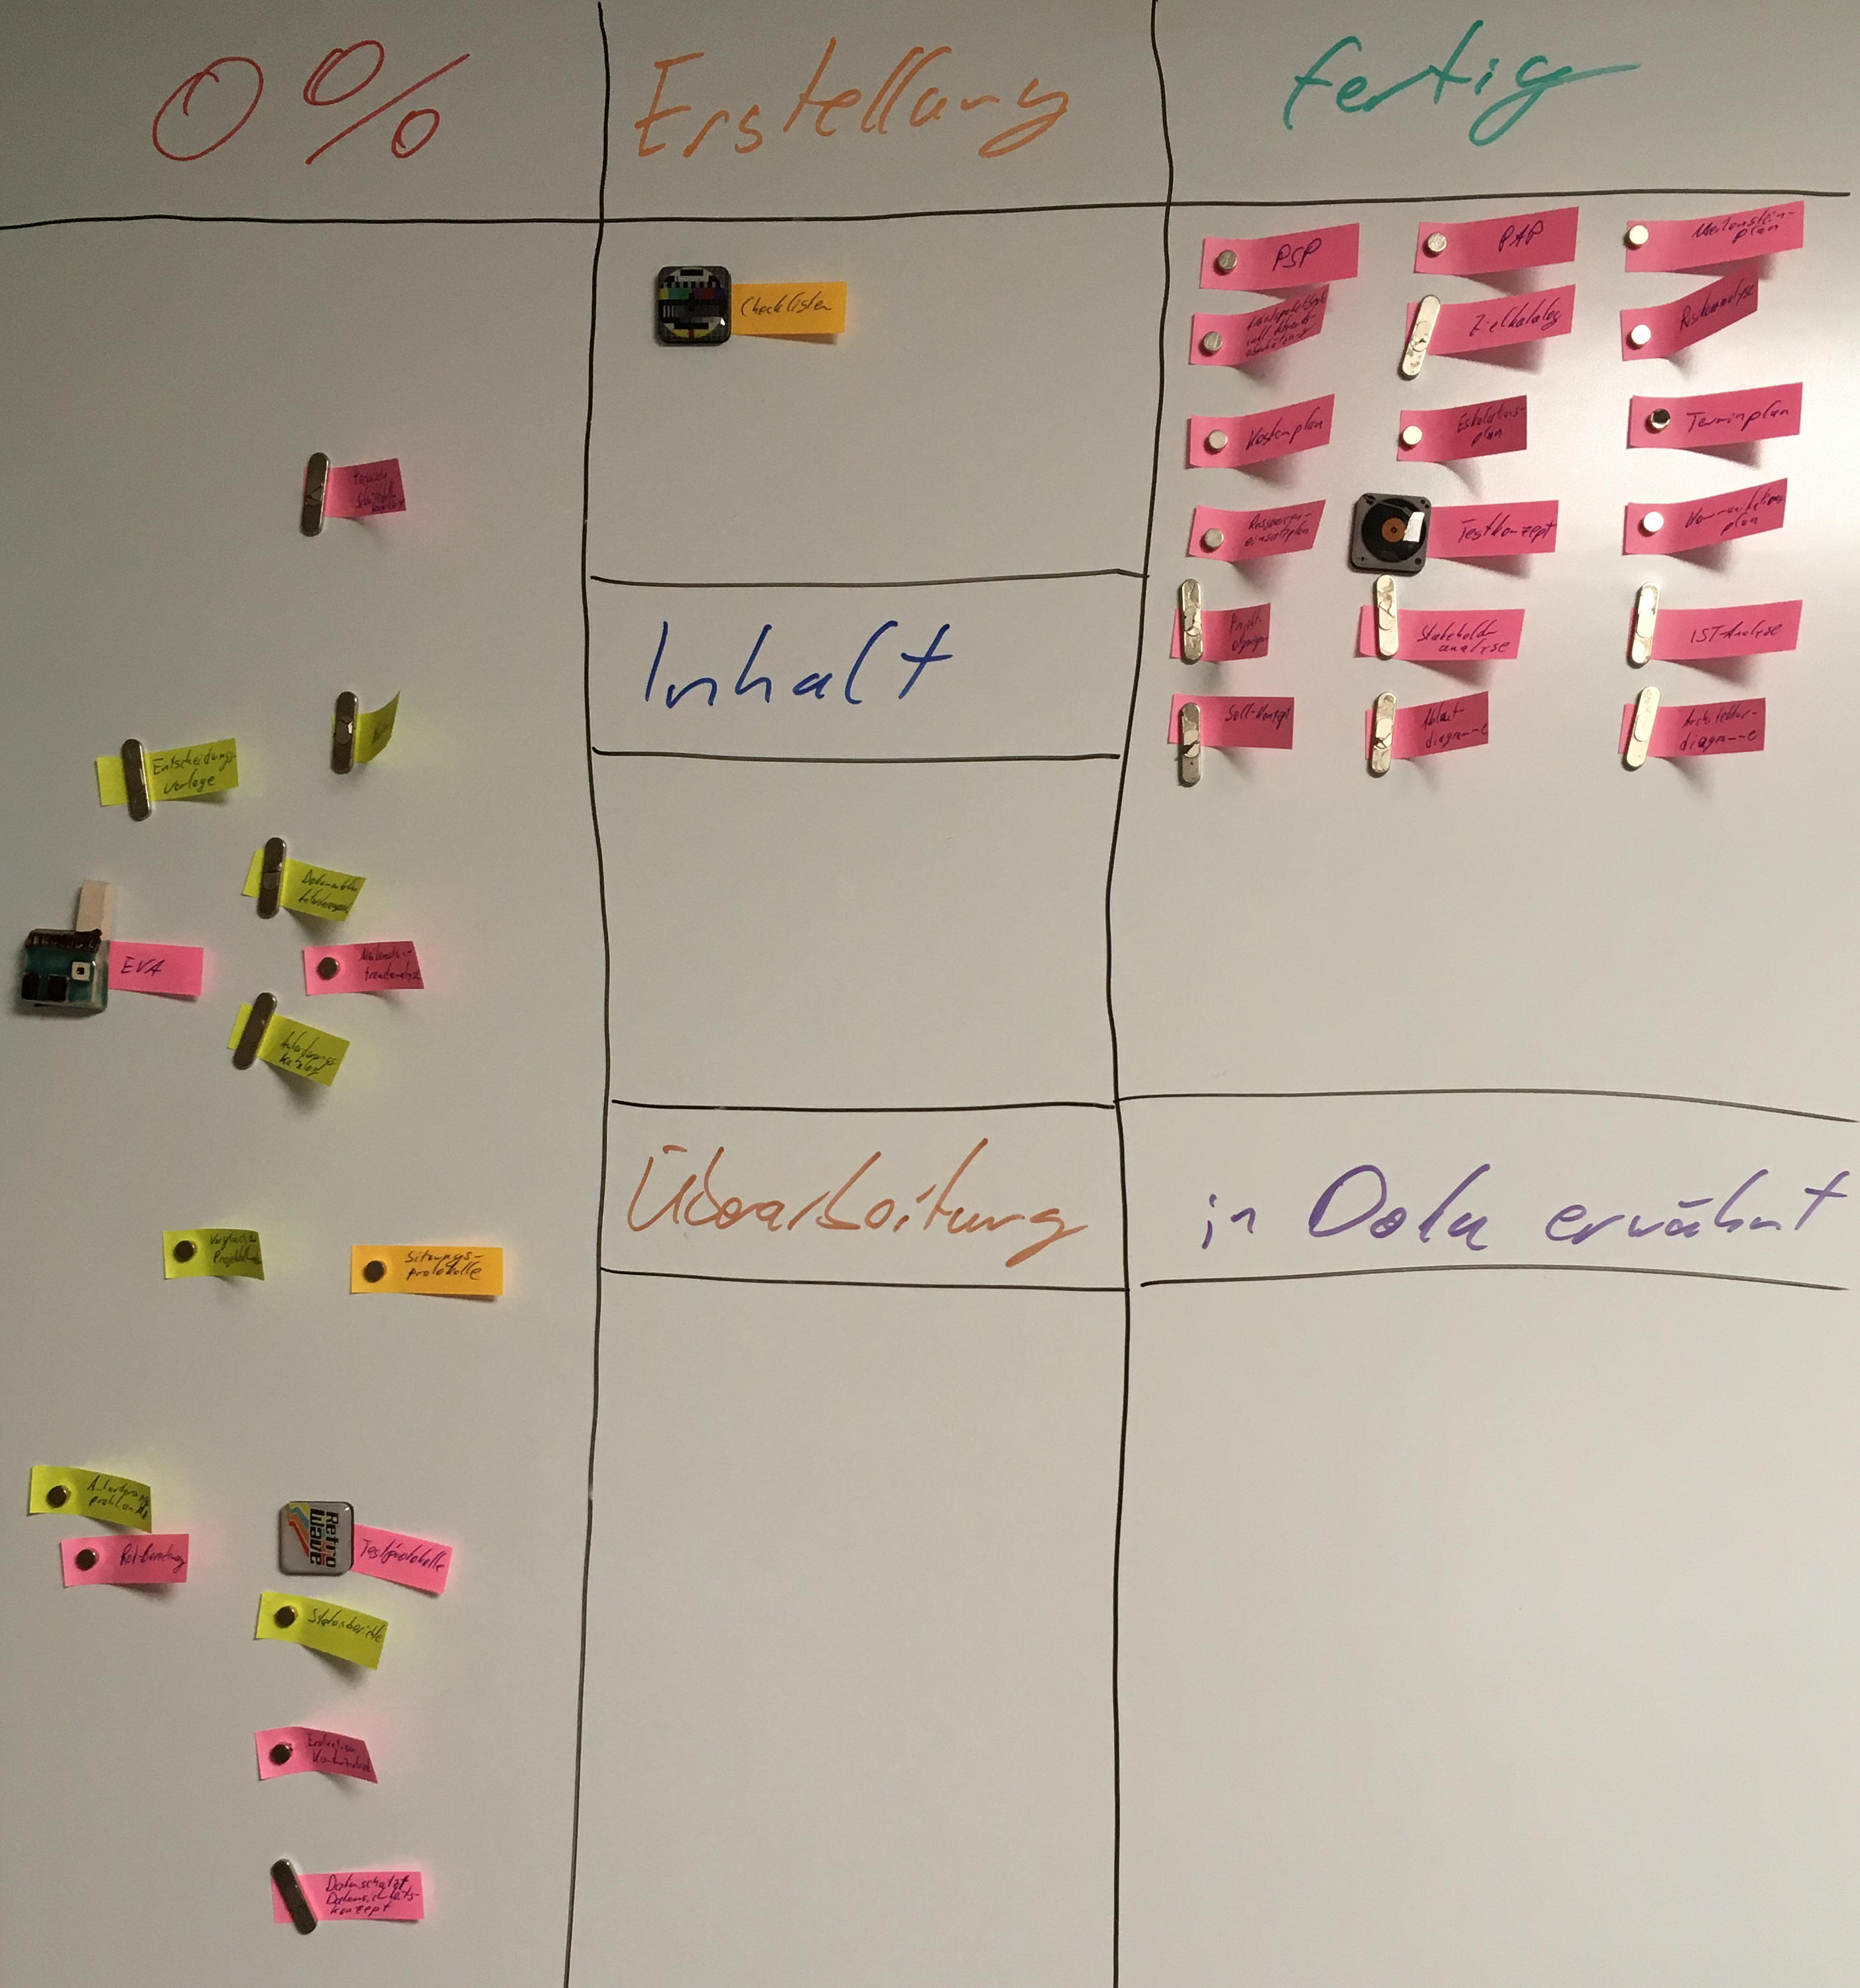
\includegraphics[width=0.85\textwidth]{./pics/kanban.jpg}
	\caption{eingebundenes Bild}
\end{figure}

Das Bild wird automatisch in das entsprechende Verzeichnis aufgenommen.

\section{Hinweis Anhänge}
Bei den Anlagen darauf achten, dass die Seitennummer immer an der richtigen Stelle ist. Also nach dem Ausdruck und der Ringheftung immer unten. Der Titel sollte hingegen immer oberhalb der \enquote{Leserichtung} dargestellt sein. Um zu verhindern, dass sich der Inhalt der Anlagen und die Überschriften der eigentlichen Dokumentation überlagern, kann mit \enquote{offset} und \enquote{scale} gearbeitet werden.
	\chapter{Kapitel Foo}
\section{Abschnitt Bar}
Lorem ipsum dolor sit amet, consetetur sadipscing elitr, sed diam nonumy eirmod tempor invidunt ut labore et dolore magna aliquyam erat, sed diam voluptua. At vero eos et accusam et justo duo dolores et ea rebum. Stet clita kasd gubergren, no sea takimata sanctus est Lorem ipsum dolor sit amet. Lorem ipsum dolor sit amet, consetetur sadipscing elitr, sed diam nonumy eirmod tempor invidunt ut labore et dolore magna aliquyam erat, sed diam voluptua. At vero eos et accusam et justo duo dolores et ea rebum. Stet clita kasd gubergren, no sea takimata sanctus est Lorem ipsum dolor sit amet. Lorem ipsum dolor sit amet, consetetur sadipscing elitr, sed diam nonumy eirmod tempor invidunt ut labore et dolore magna aliquyam erat, sed diam voluptua. At vero eos et accusam et justo duo dolores et ea rebum. Stet clita kasd gubergren, no sea takimata sanctus est Lorem ipsum dolor sit amet.   

Duis autem vel eum iriure dolor in hendrerit in vulputate velit esse molestie consequat, vel illum dolore eu feugiat nulla facilisis at vero eros et accumsan et iusto odio dignissim qui blandit praesent luptatum zzril delenit augue duis dolore te feugait nulla facilisi. Lorem ipsum dolor sit amet, consectetuer adipiscing elit, sed diam nonummy nibh euismod tincidunt ut laoreet dolore magna aliquam erat volutpat.   

\subsection{Unterabschnitt Moep}
Ut wisi enim ad minim veniam, quis nostrud exerci tation ullamcorper suscipit lobortis nisl ut aliquip ex ea commodo consequat. Duis autem vel eum iriure dolor in hendrerit in vulputate velit esse molestie consequat, vel illum dolore eu feugiat nulla facilisis at vero eros et accumsan et iusto odio dignissim qui blandit praesent luptatum zzril delenit augue duis dolore te feugait nulla facilisi.   

Nam liber tempor cum soluta nobis eleifend option congue nihil imperdiet doming id quod mazim placerat facer possim assum. Lorem ipsum dolor sit amet, consectetuer adipiscing elit, sed diam nonummy nibh euismod tincidunt ut laoreet dolore magna aliquam erat volutpat. Ut wisi enim ad minim veniam, quis nostrud exerci tation ullamcorper suscipit lobortis nisl ut aliquip ex ea commodo consequat.   

	
% --------------------------------------------------------------
% Abbildungsverzeichnis
	\clearpage
	\listoffigures
%	\addcontentsline{toc}{chapter}{\listfigurename} % Abbildungsverzeichnis ins Inhaltsverzeichnis aufnehmen

%	\listoftables % Tabellenverzeichnis
	\clearpage
%	\addcontentsline{toc}{chapter}{\listtablename}
	%Tabellenverzeichnis ins Inhaltsverzeichnis aufnehmen
	\pagenumbering{arabic}% resets `page` counter to 1
\renewcommand*{\thepage}{A\arabic{page}}

\begin{landscape}
	\appendix

	% A4 Quer
	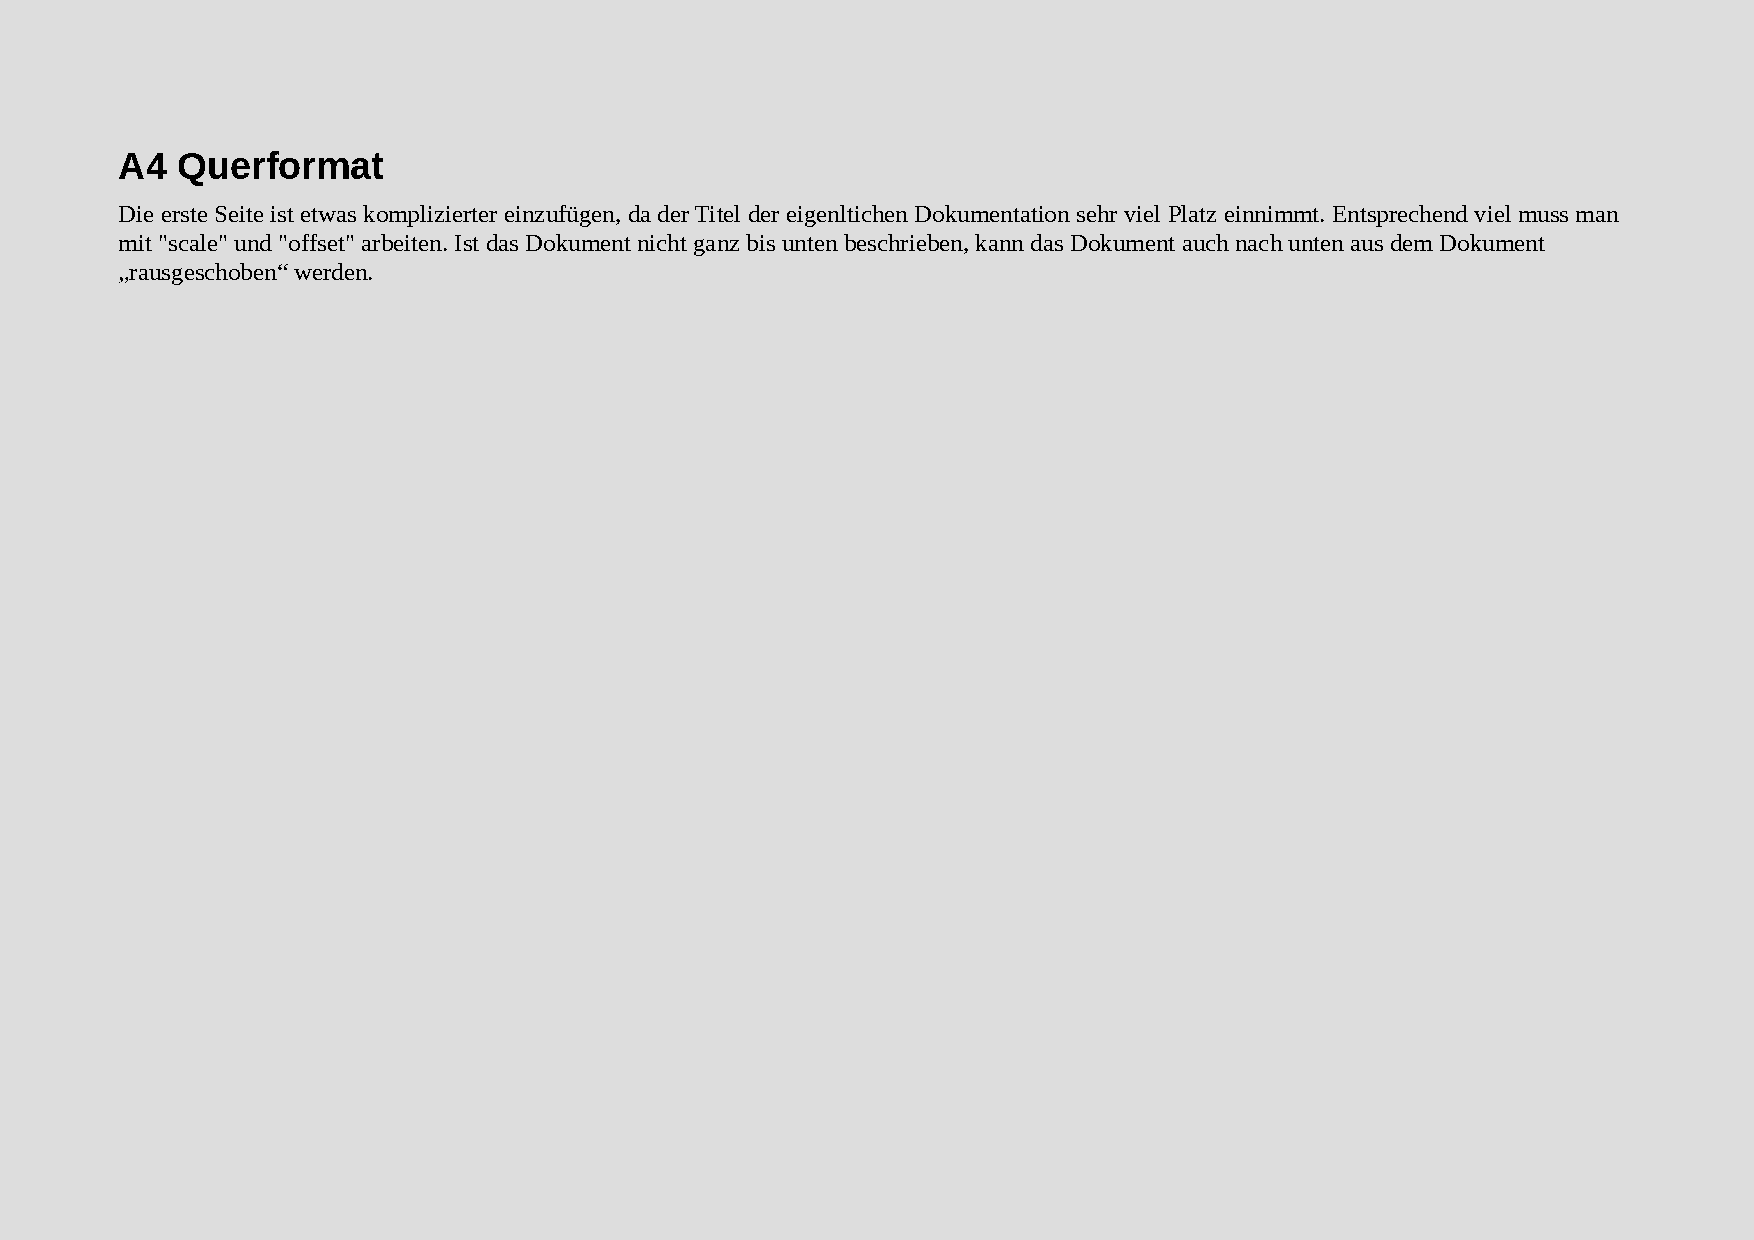
\includepdf[landscape=true,scale=1,offset=+5.5cm 0cm, pagecommand=\chapter{Anlage}\section{A4 Querformat}]{attachments/A4Querformat.pdf}

	% A3 Hoch
	
\includepdf[fitpaper,landscape=true,scale=1,offset=+1cm 0cm, pagecommand=\section{A3 Hochformat}]{attachments/A3Hochformat.pdf}

\end{landscape}

	% A4 Hoch
	
\includepdf[fitpaper,scale=1,pages=1,offset=0cm -1cm, pagecommand=\section{A4 Hochformat mehrere Seiten}]{attachments/A4Hochformat.pdf}
	
\includepdf[fitpaper,scale=1,pages=2-,offset=0cm 0cm, pagecommand={}]{attachments/A4Hochformat.pdf}

	% A3 Quer
	
\includepdf[fitpaper,landscape=false,pages=1,scale=1,offset=0 -1cm, pagecommand=\section{A3 Querformat}]{attachments/A3Querformat.pdf}


\end{document}
